% !TEX root = ../../main.tex

\section{Materials, shaping and characterisation methods}

\subsection{Materials}

In this chapter we have selected the same series of ``topical'' MOFs and 
have investigated the influence of a different shaping method, namely 
the use of alumina binder, on their adsorption properties.

The UiO-66(Zr) MOF and its derivatives are well known due to their 
stability, both in regards to temperature and chemical 
compounds~\cite{cavkaNewZirconiumInorganic2008}. It is composed of
Zr6-oxo clusters which are connected with benzene dicarboxilate 
(BDC) linkers to form a face-centered cubic framework. It has 
shown promise~\cite{wiersumEvaluationUiO66GasBased2011}
in use for gas adsorption applications.

MIL-100(Fe) is a MOF which uses the benzene tricarboxilate (BTC) linker 
in conjunction with trimeric iron (III) octahedral clusters
~\cite{horcajadaSynthesisCatalyticProperties2007,
YangWaterStableMetalOrganic2013}.
The framework assembles in hybrid supertetrahedra which leads to very 
large pore sizes. The iron trimers are coordinated with
anions and have shown a propensity to partially reduce to a divalent 
\ce{Fe^2+} state, exposing a naked metal site in the process.
~\cite{yoonControlledReducibilityMetalOrganic2010}

The last material, MIL-127(Fe), originally reported 
by~\citeauthor{liuAssemblyMetalOrganic2007} is a MOF built from the same
metal (III) octahedra trimers as MIL-100(Fe), but using the
3,3',5,5'-azobenzenetetracarboxylate (TazBz) linker, to produce a 
framework with the (soc) topology. This material has shown 
promise~\cite{chevreauSynthesisBiocompatibleHighly2016}
for large scale synthesis. Furthermore, due to its alternating
hydrophobic/hydrophilic microporous systems, it has been shown to be
of interest for multiple applications such as catalysis or 
\ce{CO2} capture~\cite{chanutScreeningEffectWater2017}.

The UiO-66(Zr) and MIL-100(Fe) powders have been synthesised at the
Korea Research Institute of Chemical Technology (KRICT).
The MIL-127(Fe) MOF was made in the group of Christian Serre,
in the Lavoisier Institute in Versailles.
Complete details of the synthesis method can be found in the related
publication~\cite{valekarShapingPorousMetal2017}
and in Appendix~\ref{appx:synthesis}.
The structures of the three materials can be seen 
in \autoref{shaping:fgr:mofstructures}.


\begin{figure}[htb]
	\centering
	\begin{subfigure}{0.3\textwidth}
		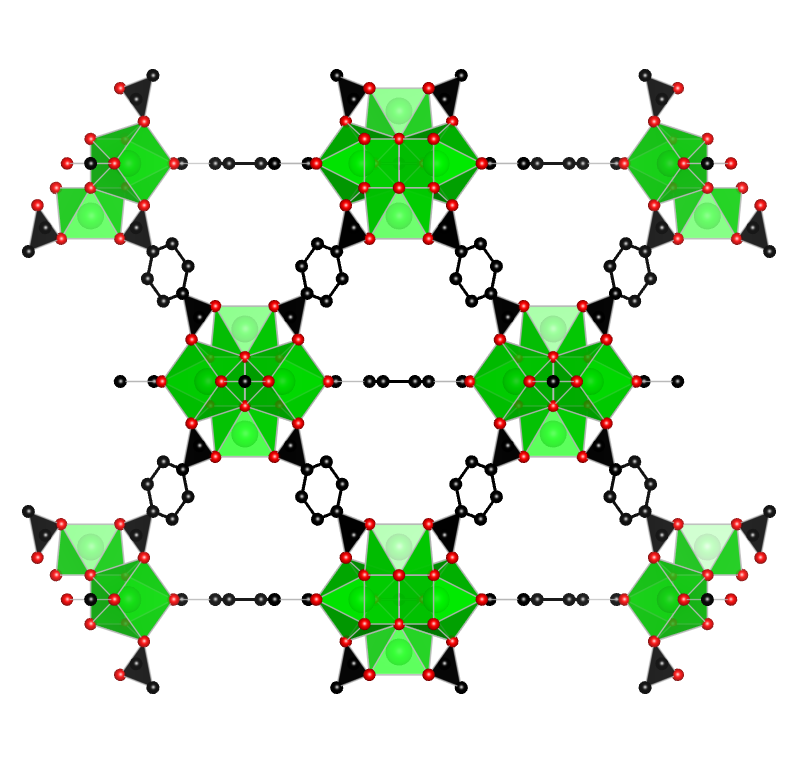
\includegraphics[width=\linewidth]{structure/uio66}
		\caption{UiO-66(Zr)}
	\end{subfigure}
	\begin{subfigure}{0.3\textwidth}
		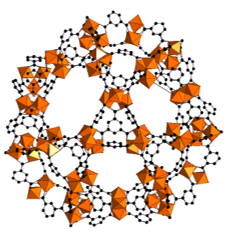
\includegraphics[width=\linewidth]{structure/mil100}
		\caption{MIL-100(Fe)}
	\end{subfigure}
	\begin{subfigure}{0.3\textwidth}
		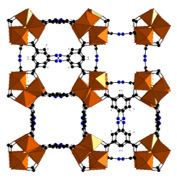
\includegraphics[width=\linewidth]{structure/mil127}
		\caption{MIL-127(Fe)}
	\end{subfigure}

	\caption{The unit structures of the investigated MOFs.
		The colour coding is as follows: Zr polyhedra in green,
		Fe octahedra in brown, C in black, O in red, N in blue.
		Hydrogen atoms are omitted for clarity.}%
	\label{shaping:fgr:mofstructures}
\end{figure}




\subsection{Shaping Procedure}

The shaping of the samples also took place at KRICT and was done
using a wet granulation method. In the case of the alumina binder,
the MOF powder was was mixed with the previously prepared mesoporous
\(\rho\)-alumina with water added as the dispersing medium. For the
PVA binder, the MOF powder was instead added to a solution of
ethanol solution containing a polymer mixture of polyvinyl groups
such as polyvinyl alcohol and polyvinyl butyral. The resulting
mixture was shaped into beads using a hand-made pan granulator.
During the process, the spheres were sprayed with the respective
solvent in order to achieve desired size. The beads were then sieved
and rolled using a roller machine to enhance their spherical
shape. Finally, the prepared samples were dried at \SI{303}{\kelvin}
for \SI{12}{\hour} to remove all residual solvent.
The resulting beads were near spherical in shape, with a diameter
between \SIrange{2}{2.5}{\milli\metre}.

\subsection{Characterisation of powders and pellets}

The primary interest of the study was observing differences
in adsorption properties between the powder and the shaped materials.

Thermogravimetric analysis was used to verify that the binder
did not change the thermal stability of the materials and, in the
case of the PVA variant, to ensure that the activation temperature
chosen did not induce polymer decomposition. The TGA method is described
in detail in Appendix~\ref{appx:char:TGA}.

The bulk and skeletal density of the powder and pellets were measured
to allow isotherms to be presented on a volume basis, as well as
to check the level of densification afforded through the
shaping process. The procedure is described in Appendix~\ref{appx:char:bulkdensity} and Appendix~\ref{appx:char:truedensity}.

Specific surface area and pore volume were determined through
nitrogen adsorption at \SI{77}{\kelvin}. These measurements were
recorded according to the method in Appendix~\ref{appx:char:N2phys}.
For inspecting changes in surface hydrophobicity, water and
methanol adsorption isotherms were measured according to
the method presented in Appendix~\ref{appx:char:vapourphys}.

Finally, all calorimetry data was recorded using the high sensitivity
Tian-Calvet calorimeter coupled with adsorption volumetry, as
introduced in \autoref{calo}.

\subsection{Sample activation for adsorption}

The materials were pre-treated before all adsorption experiments by
activation at high temperature under secondary vacuum for 16 hours.
The activation temperature was specific
to each solid: \SI{200}{\degreeCelsius} for UiO-66(Zr),
\SI{150}{\degreeCelsius} for MIL-100(Fe) and \SI{150}{\degreeCelsius}
for MIL-127(Fe).
